\section{Durchführung}
\label{sec:Durchfuehrung}

\begin{figure}[H]
  \centering
  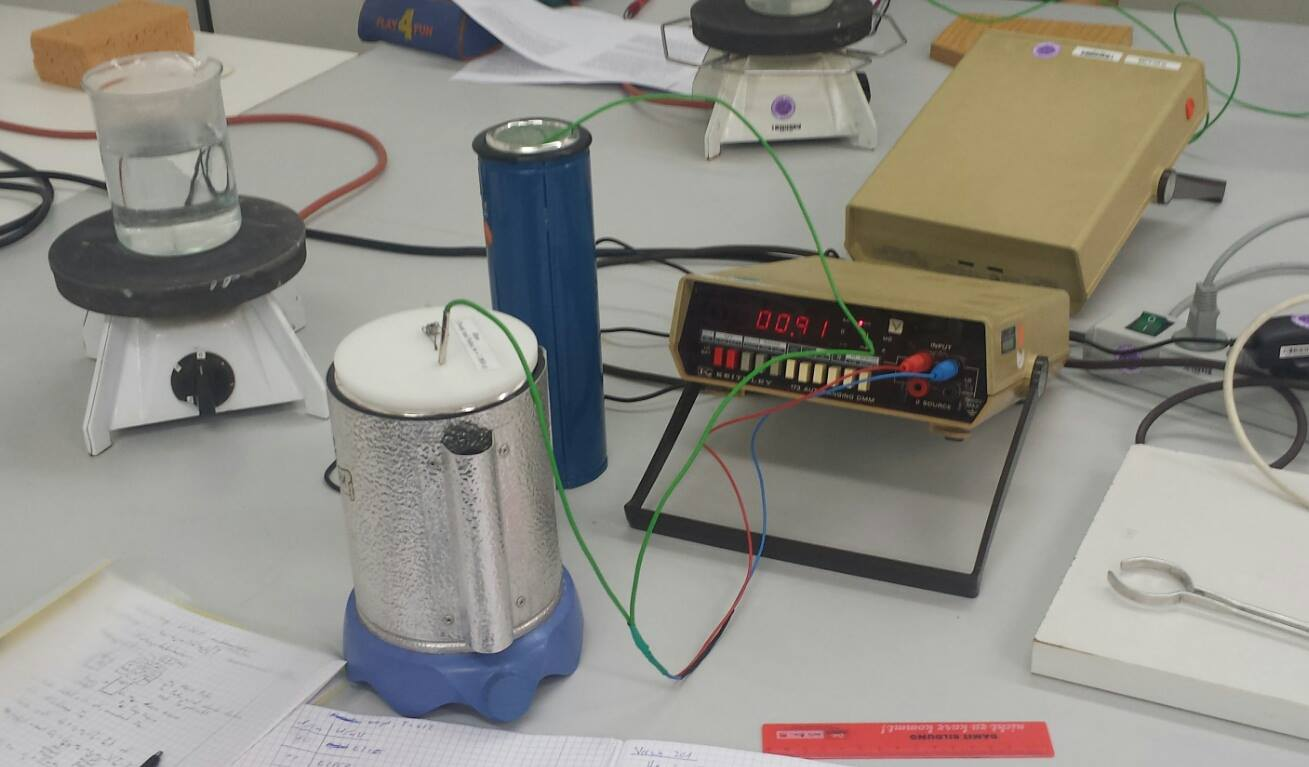
\includegraphics[height=6cm]{aufbau.png}
  \caption{Versuchsaufbau.}
  \label{fig:aufbau}
\end{figure}


Die Bestimmung der spezifischen Wärmekapazität $c_k$ der Festkörper erfolgt mittels Mischungskalometrie.
\subsection{Bestimmung der Wärmekapazität des Kalorimeters}
Damit die Mischungskalometrie für die Festkörper durchgeführt werden kann, muss zunächst die Wärmekapazität $c_g \cdot m_g$ des Kalorimeters bestimmt werden.
Dieses besteht aus einem Dewargefäß, welches thermisch isoliert ist. \\
Es werden nun zwei in etwa gleich große, abgemessene Mengen Wasser benötigt.
Die erste Menge wird in das Dewargefäß gefüllt, so dass dieses die gleiche Temperatur $T_1$ wie die Außenwände erhält.
Die zweite Menge wird auf einer Heizplatte auf eine Temperatur $T_2$ erwärmt.
Beide Mengen werden nun im Dewargefäß gemischt, bis sich eine konstante Mischtemperatur $T_m$ eingestellt hat.
Damit sich im Gefäß eine gleichmäßige Temperaturverteilung ergibt, wird das Wasser mithilfe eines rotierenden Magnetrührstäbchens umgerührt. \\
Aus den Werten $T_1$, $T_2$, $T_m$, den Gewichten des Wassers und der spezifischen Wärmekapazität vom Wasser ergibt sich die Wärmekapazität des Kalorimeters \ref{eqn:7}. \\
Es ist darauf zu achten, dass bei der Messung die Füllhöhe des Dewargefäßes in etwa mit der Füllhöhe im späteren Versuchsverlauf übereinstimmt, da ansonsten Abweichungen auftreten können.

\subsection{Bestimmung der spezifischen Wärmekapazität}
Zunächst wird die Masse der zu untersuchende Probe mittels einer Schnellwaage zu $m_k$ bestimmt.
Um die Probe nun zu erwärmen, wird diese in ein mit Wasser gefülltes Becherglas getaucht und auf eine Heizplatte gestellt.
Der Körper erhält nun eine Temperatur von $T_k$. \\
Die Temperaturmessung wird dabei mit einem Thermoelement durchgeführt.
Dieses besteht aus zwei Kontaktstellen, von denen eine in Eiswasser gelegt wird, dessen Temperatur \SI{0}{\celsius} ist.
Die andere Kontaktstelle wird an dem zu messenden Probekörper befestigt.
Aus der entstehenden Thermospannung $U_{th}$ lässt sich die Temperaturdifferenz berechnen. \\
Gleichzeitig wird eine zu $m_w$ abgemessene Menge Wasser in das Dewargefäß gefüllt.
Dessen Temperatur wird kurz vor dem Mischvorgang mithilfe des Thermoelementes zu $T_w$ bestimmt.
Nun wird der Probekörper aus dem Becherglas genommen und in das Dewargefäß gestellt.
Es wird gewartet, bis der Temperaturausgleich abgeschlossen ist und sich eine feste Mischtemperatur $T_m$ eingestellt hat. \\
Aus den Massen $m_w$ und $m_k$, den Temperaturen $T_k$, $T_w$ und $T_m$ sowie den Wärmekapazitäten $c_g \cdot m_g$ und $c_w$ kann die spezifische Wärmekapazität der Probe berechnet werden \ref{eqn:7}.
Durch Kenntnis der Stoffmenge $n$ des Materials lässt sich somit die gesuchte Molwärme ermitteln \ref{eqn:6}.  \\
